% !TeX program = xelatex
% !TeX encoding = UTF-8
\documentclass[UTF8]{standalone}
\usepackage{amsmath,fourier,ctex,tikz}
\begin{document}
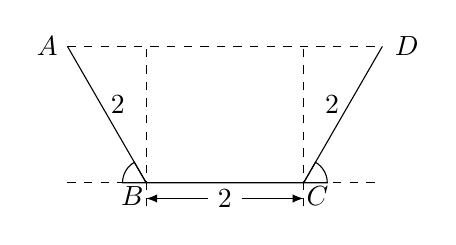
\begin{tikzpicture}
	\draw (0,0) node[left=5pt,below=-2pt] {$B$} -- node[right=4pt,above=-3pt] {$2$} ++ (120:2) node[left] {$A$} ++ (-60:2) -- ++ (2,0) node[right=5pt,below=-2pt] {$C$} -- node[left=4pt,above=-3pt] {$2$} ++ (60:2) node[right=1pt] {$D$};
	\draw[dashed] (0,0) ++ (120:2) -- ++ (4,0);
	\draw[dashed] (0,-0.3) -- ++ (0,2.0320);
	\draw[dashed] (2,-0.3) -- ++ (0,2.0320);
	\draw[dashed] (-1,0) -- (3,0);
	\node (a) at (1,-0.2) {$2$};
	\draw[latex-] (0,-0.2) -- (a);
	\draw[-latex] (a) -- (2,-0.2);
	\draw (2,0) -- ++ (0.3,0) arc [start angle=0, end angle=60, radius=0.3] -- cycle;
	\draw (0,0) -- ++ (-0.3,0) arc [start angle=180, end angle=120, radius=0.3] -- cycle;
\end{tikzpicture}
\end{document}